%%% Ne pas modifier jusqu'à la ligne 25
\documentclass[a4paper,12pt]{book}
\usepackage[utf8]{inputenc}
\usepackage[french]{babel}
%%\usepackage{CJK}
\usepackage{yhmath}
\usepackage[left=2cm,right=2cm,top=3cm,bottom=2cm, headheight=1.5cm,headsep=1.5cm]{geometry}
%%\usepackage{CJKutf8}
\usepackage{amsfonts}
\usepackage{mathrsfs}
\usepackage{amsmath,amsfonts,amssymb,dsfont}
\usepackage{graphicx}
\usepackage{subfigure}
\usepackage{enumitem}		%\enumerate-resume
\usepackage[colorlinks=true,unicode={true},hyperindex=false, linkcolor=blue, urlcolor=blue]{hyperref}
\newcommand{\myref}[1]{\ref{#1} page \pageref{#1}}

\addto\captionsfrench{\def\tablename{Tableau}}  %légendes des tableaux
\renewcommand\thesection{\Roman{section}~-~} 
\renewcommand\thesubsection{\Roman{section}.\Alph{subsection}~-~} 
\renewcommand\thesubsubsection{\Roman{section}.\Alph{subsection}.\arabic{subsubsection}~-~} 

\newcommand{\conclusion}[1]{\newline \centerline{\fbox{#1}}}

\setcounter{secnumdepth}{3}
\parindent=0pt

\usepackage{fancyhdr}
\pagestyle{fancy}

\lhead{SJTU-ParisTech} 
%%%%%%%%%%%%%%%%%%%%%%%%%%%%%%%%%%
\chead{DM3}
\rhead{Daniel 518261910024}

\begin{document}
\renewcommand{\labelitemi}{$\blacktriangleright$}
\renewcommand{\labelitemii}{$\bullet$}


\section{Activité 2-3}
\begin{figure}[h]
    \begin{center}
    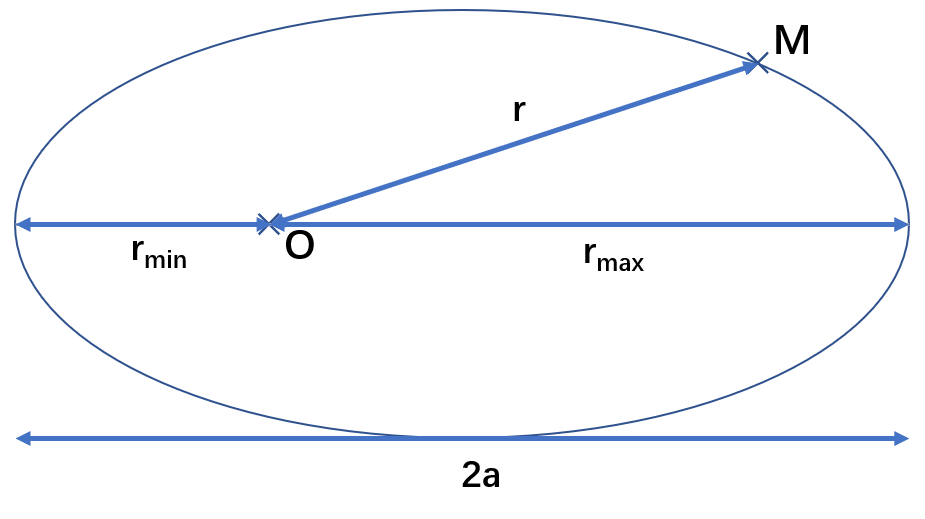
\includegraphics[scale=0.6]{meca31.png}
    \end{center}
    \caption{le système étudiée}
\end{figure}
\subsection{}
Pour un point matériel $M$ de masse $m$ suivant une force conservative centrale, on a 
$$
E_m=\frac{1}{2}m\dot{r}^2+E_{p,eff}(r)
$$
avec
$$
E_{p,eff}(r)=E_p(r)+\frac{L_O^2}{2mr^2}
$$ 
où $r=\Vert\overrightarrow{OM}\Vert$, $L_O$ le norme du mouvement cinétique.

Lorsque $r=r_{min}$ ou $r=r_{max}$, on a $\dot{r}=0$, et l'énergie potentielle est donnée par $E_p(r)=-\frac{K}{r}$, $K$ est une constante. 

On a donc $r_{min}$ et $r_{max}$ sont les deux raccines de cette équation
$$
E_m=E_{p,eff}(r)=-\frac{K}{r}+\frac{L_O^2}{2mr^2}
$$
soit
$$
E_m\times r^2+K\times r-L_O^2=0
$$
donc on a 
$$
r_{min}+r_{max}=-\frac{K}{E_m}
$$
Comme $r_{min}+r_{max}=2a$, où $a$ est le demi-grand
axe de l'ellipse, on a finalement 
$$
\boxed{E_m=-\frac{K}{2a}}
$$
\section{Exercice 2-7}
\begin{figure}[h]
    \begin{center}
    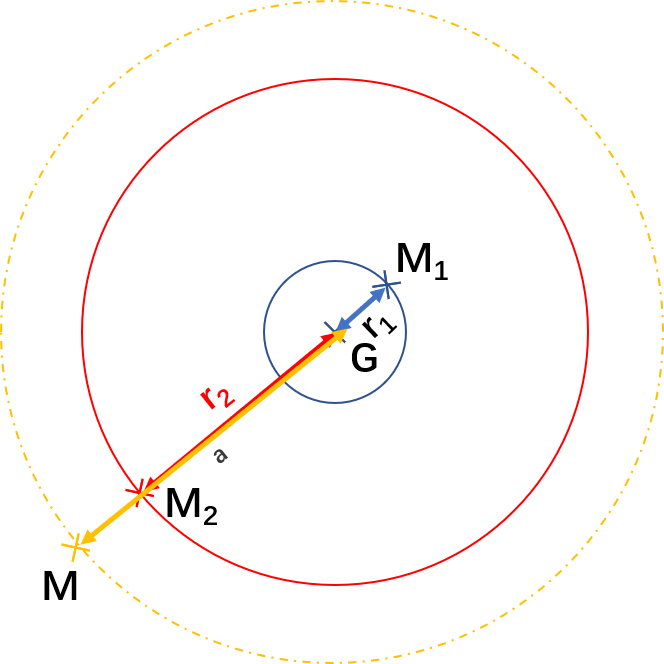
\includegraphics[scale=0.6]{meca32.png}
    \end{center}
    \caption{le système étudiée}
\end{figure}
Considerons le système Terre-Soliel, puisque $m_{terre} \ll m_{soleil}$, on a donc l'approximation
$$
\frac{T_{t-s}^2}{a_{t-s}^3}=\frac{4\pi^2}{Gm_{soliel}}
$$
avec $T_{t-s} \simeq 1\,ans$ la période de révolution, et $a_{t-s}= 1$ unité astronomique, 
on en déduit la constante gravitationnelle
$$
G=\frac{4\pi^2a_{t-s}^3}{T_{t-s}^2m_{soleil}}
$$
Pour le système $(\Sigma)$ des deux étoiles $(M_1,m_1)$ et $(M_2,m_2)$, on sait que il tourne autour de leur barycentre $G$, 
on a donc 
$$
\overrightarrow{GM_1}=\frac{-m_2}{m_1+m_2}\overrightarrow{GM}
$$
où $M$ est la particule fictive vérifiant $\overrightarrow{GM}=\overrightarrow{M_1M_2}$, donc 
$$
|\frac{-m_2}{m_1+m_2}|=\frac{\Vert\overrightarrow{GM_1}\Vert}{\Vert\overrightarrow{GM}\Vert}=\frac{r_1}{r_1+r_2}
$$
on a donc $m_1=5m_2$

On sait que le point $M$ vérifie 
$$
\frac{T_{M}^2}{a_{M}^3}=\frac{4\pi^2}{G(m_1+m_2)}
$$
avec $T_{M}=20ans$, $a_{M}=\Vert\overrightarrow{GM}\Vert=18$ unités astronomiques, donc 
$$
m_1+m_2=\frac{4\pi^2a_{M}^3}{GT_{M}^2}
$$
A.N.
$$
m_1+m_2=\frac{a_{M}^3T_{t-s}^2m_{soleil}}{a_{t-s}^3T_{M}^2}=\frac{18^3}{20^2}\,m_{soleil}=14.58\,m_{soleil}
$$
On a donc $\boxed{m_1=12.15\,m_{soleil}, m_2=2.43\,m_{soleil}}$
\end{document}